\documentclass[a4paper]{book}

\usepackage{amsmath}
\usepackage{amssymb}
\usepackage[hypcap=false]{caption}
\usepackage{enumitem}	% 定制enumerate标号
\usepackage{geometry}
\geometry{
	left=2cm,
	right=2cm,
	top=2cm,
	bottom=2cm,
}
\usepackage{hyperref}
\hypersetup{
    colorlinks=true,            %链接颜色
    linkcolor=blue,             %内部链接
    filecolor=magenta,          %本地文档
    urlcolor=cyan,              %网址链接
}
\usepackage[none]{hyphenat}		% 阻止长单词分在两行
\usepackage{mathrsfs}
\usepackage{mathtools}
\usepackage[version=4]{mhchem}
\usepackage{subcaption}
\usepackage{titlesec}

\RequirePackage[many]{tcolorbox}
\tcbset{
    boxed title style={colback=magenta},
	breakable,
	enhanced,
	sharp corners,
	attach boxed title to top left={yshift=-\tcboxedtitleheight,  yshifttext=-.75\baselineskip},
	boxed title style={boxsep=1pt,sharp corners},
    fonttitle=\bfseries\sffamily,
}

\definecolor{skyblue}{rgb}{0.54, 0.81, 0.94}

\newtcolorbox[auto counter, number within=chapter, number format=\arabic]{exercise}[1][]{
    title={Exercise~\thetcbcounter},
    colframe=skyblue,
    colback=skyblue!12!white,
    boxed title style={colback=skyblue},
    overlay unbroken and first={
        \node[below right,font=\small,color=skyblue,text width=.8\linewidth]
        at (title.north east) {#1};
    }
}

\newtcolorbox[auto counter, number within=chapter, number format=\arabic]{solution}[1][]{
    title={Solution~\thetcbcounter},
    colframe=teal!60!green,
    colback=green!12!white,
    boxed title style={colback=teal!60!green},
    overlay unbroken and first={
        \node[below right,font=\small,color=red,text width=.8\linewidth]
        at (title.north east) {#1};
    }
}

% special new commands for common symbols used in the article
\newcommand\la{\langle}
\newcommand\ra{\rangle}
\newcommand\lr[2]{\langle#1\|#2\rangle}
\newcommand\tr[1]{\mathrm{tr(#1)}}
\newcommand\Tr[3]{#1\mathrm\#2#3}
\newcommand*{\dif}{\mathop{}\!\mathrm{d}}
\renewcommand\det[1]{\mathrm{det\left(#1\right)}}
\newcommand{\HF}{{\rm HF}}
\newcommand{\bfr}{{\bf r}}

\newcommand{\A}{{\bf A}}
\newcommand{\B}{{\bf B}}
\newcommand{\C}{{\bf C}}
\newcommand{\I}{{\bf 1}}
\newcommand{\U}{{\bf U}}
\newcommand{\Op}{{\bf O}}

\titleformat{\chapter}[display]
  {\bfseries\Large}
  {\filright\MakeUppercase{\chaptertitlename} \Huge\thechapter}
  {1ex}
  {\titlerule\vspace{1ex}\filleft}
  [\vspace{1ex}\titlerule]
  
\allowdisplaybreaks

\begin{document}

	\stepcounter{chapter}

	\chapter{Many Electron Wave Functions and Operators}
	
	\section{The Electron Problem}
	
	\subsection{Atomic Units}
	
	\subsection{The Born-Oppenheimer Approximation}
	
	\subsection{The Antisymmetry or Pauli Exclusion Principle}
	
	\section{Orbitals, Slater Determinants, and Basis Functions}
	
	\subsection{Spin Orbitals and Spatial Orbitals}
	
	\begin{exercise}
	Given a set of $K$ orthonormal spatial functions, $\{\psi^\alpha_i(\bfr)\}$, and another set of $K$ orthonomal functions, $\{\psi^\beta_i(\bfr)\}$, such that the first set is not orthogonal to the second set, i.e, 
	\[
		\int \dif \bfr \psi^{\alpha*}_i( \bfr ) \psi^\beta_j( \bfr ) = S_{ij}
	\]
	where ${\bf S}$ is an overlap matrix, show that the set $\{ \chi_i \}$ of $2K$ spin orbitals, formed by multiplying $\psi^\alpha_i( \bfr )$ by the $\alpha$ spin function and $\psi^\beta_i( \bfr )$ by the $\beta$ spin function, i.e.,
	\[
	\begin{dcases}
		\chi_{2i-1} &= \psi^\alpha_i( \bfr ) \alpha( \omega ) \\
		\chi_{2i} &= \psi^\beta_i( \bfr ) \beta( \omega )
	\end{dcases} i = 1, 2, \ldots, K
	\]
	is an orthonormal set.
	\end{exercise}
	
	\begin{solution}
		2-1 so
	\end{solution}
	
	\subsection{Hartree Products}
	
	\begin{exercise}
	Show that the Hartree product of (2.30) is an eigenfunction of $\mathscr{H} = \sum_{i=1}^N h(i)$ with an eigenvalue given by (2.32).
	\end{exercise}
	
	\begin{solution}
		2-2 so
	\end{solution}
	
	\subsection{Slater Determinants}
	
	\begin{exercise}
	Show that $\Psi({\bf x}_1,{\bf x}_2)$ of Eq.(2.34) is normalized.
	\end{exercise}
	
	\begin{solution}
		2-3 so
	\end{solution}

	\begin{exercise}
	Suppose the spin orbitals $\chi_i$ and $\chi_j$ are eigenfunctions of a one-electron operator $h$ with eigenvalues $\varepsilon_i$ and $\varepsilon_j$ as in Eq.(2.29). Show that the Hartree products in Eqs.(2.33a, b) and the antisymmetrized wave function in Eq.(2.34) are eigenfunctions of the independent-particle Hamiltonian $\mathscr{H} = h(1) + h(2)$ (c.f. Eq.(2.28)) and have the same eigenvalue namely, $\varepsilon_i + \varepsilon_j$. 
	\end{exercise}
	
	\begin{solution}
		2-4 so
	\end{solution}
	
	\begin{exercise}
	Consider the Slater determinants
	\[
		| K \rangle = | \chi_i \chi_j \rangle, \quad | L \rangle = | \chi_k \chi_l \rangle.
	\]
	Show that
	\[
		\langle K | L \rangle = \delta_{ik} \delta_{jl} - \delta_{il} \delta_{jk}.
	\]
	Note that the overlap is zero unless: 1) $k=i$ and $l=j$, in which case $|L\rangle$ = $|K\rangle$ and the overlap is unity and 2) $k=j$ and $l=i$ in which case $|L\rangle= |\chi_j \chi_i \rangle = -|K\rangle$ and the overlap is minus one.
	\end{exercise}
	
	\begin{solution}
		2-5 so
	\end{solution}
	
	\subsection{The Hartree-Fock Approximation}
	
	\subsection{The Minimal Basis \texorpdfstring{$\ce{H2}$}- Model}
	
	\begin{exercise}
	Show that $\psi_1$ and $\psi_2$ form an orthonormal set.
	\end{exercise}
	
	\begin{solution}
		2-6 so
	\end{solution}
	
	\subsection{Excited Determinants}
	
	\subsection{Form of the Exact Wave Function and Configuration Interaction}
	
	\begin{exercise}
	A minimal basis set for benzene consists of 72 spin orbitals. Calculate the size of the full CI matrix if it would be formed from determinants. How many singly excited determinants are there? How many doubly excited determinants are there?
	\end{exercise}
	
	\begin{solution}
		2-7 so
	\end{solution}
	
	\section{Operators and Matrix Elements}
	
	\subsection{Minimal Basis \texorpdfstring{$\ce{H2}$}- Matrix Elements}
	
	\begin{exercise}
	Show that
	\[
		\langle \Psi^{34}_{12} | \mathscr{O}_1 | \Psi^{34}_{12} \rangle = \langle 3 | h | 3 \rangle + \langle 4 | h | 4 \rangle
	\]
	and
	\[
		\langle \Psi_0 | \mathscr{O}_1 | \Psi^{34}_{12} \rangle = \langle \Psi^{34}_{12} | \mathscr{O}_1 | \Psi_0 \rangle = 0.
	\]
	\end{exercise}
	
	\begin{solution}
		2-8 so
	\end{solution}
	
	\begin{exercise}
	Using the above approach, show that the full CI matrix for minimal basis $\ce{H2}$ is
	\[
		\mathscr{H} = \begin{pmatrix}
			\langle 1 | h | 1 \rangle + \langle 2 | h | 2 \rangle + \langle 12 | 12 \rangle - \langle 12 | 21 \rangle & \langle 12 | 34 \rangle - \langle 12 | 43 \rangle \\
			\langle 34 | 12 \rangle - \langle 34 | 21 \rangle & \langle 3 | h | 3 \rangle + \langle 4 | h | 4 \rangle + \langle 34| 34 \rangle - \langle 34 | 43 \rangle
		\end{pmatrix}.
	\]
	and that is it Hermitian.
	\end{exercise}
	
	\begin{solution}
		2-9 so
	\end{solution}
	
	\subsection{Notations for One- and Two-Electron Integrals}
	
	\subsection{General Rules for Matrix Elements}
	
	\begin{exercise}
	Derive Eq.(2.110) from Eq.(2.107).
	\end{exercise}
	
	\begin{solution}
		2-10 so
	\end{solution}
	
	\begin{exercise}
	If $|K\rangle = |\chi_1 \chi_2 \chi_3 \rangle$ show that
	\[
		\langle K | \mathscr{H} | K \rangle = \langle 1 | h | 1 \rangle + \langle 2 | h | 2 \rangle + \langle 3 | h | 3 \rangle + \lr{12}{12} + \lr{13}{13} + \lr{23}{23}.
	\]
	\end{exercise}
	
	\begin{solution}
		2-11 so
	\end{solution}
	
	\begin{exercise}
	Evaluate the matrix elements that occur in the minimal basis $\ce{H2}$ full CI matrix (Eq.(2.79)) using the rules. Compare with the result obtained in Exercise 2.9.
	\end{exercise}
	
	\begin{solution}
		2-12 so
	\end{solution}
	
	\begin{exercise}
	Show that
	\[ \langle \Psi^r_a| \mathscr{O}_1 | \Psi^s_b \rangle =
	\begin{dcases}
		0, & \text{if } a \neq b , \, r \neq s ; \\ 
		\langle r | h | s \rangle, & \text{if } a = b , \, r \neq s ; \\ 
		-\langle b | h | a \rangle, & \text{if } a \neq b , \, r = s ; \\
		\sum_c^N \langle c | h | c \rangle - \langle a | h | a \rangle + \langle r | h | r \rangle & \text{if } a = b , \, r = s. 
	\end{dcases}
	\]	
	\end{exercise}
	
	\begin{solution}
		2-13 so
	\end{solution}
	
	\begin{exercise}
	The Hartree-Fock ground state energy for an $N$-electron system is $^N E_0 = \langle ^N \Psi_0 | \mathscr{H} | ^N \Psi_0 \rangle$. Consider a state of the ionized system (in which an electron has been removed from spin orbital $\chi_a$) with energy $^{N-1} E_a = \langle ^{N-1} \Psi_a | \mathscr{H} | ^{N-1} \Psi_a \rangle$, where $| ^{N-1} \Psi_a \rangle$ is a single determinant with all spin orbitals but $\chi_a$ occupied,
	\[
		| ^{N-1} \Psi_a \rangle = | \chi_1 \chi_2 \cdots \chi_{a-1} \chi_{a+1} \cdots \chi_N \rangle.
	\]
	Show, using the rules in the tables, that the energy required for this ionization process is
	\[
		^N E_0 - ^{N-1} E_a = \langle a | h | a \rangle + \sum_b^N \lr{ab}{ab}.
	\]
	To show the power and simplicity of the mnemonic device introduced in this subsection, let us derive the above result without doing any algebra. Consider the representation of $|^N \Psi_0 \rangle$ in Fig. 2.4. If we remove an electron from $\chi_a$, we lose the ``one-electron energy" contribution $\langle a | h | a \rangle$ to $^N E_0$. Moreover, we lose the pair-wise contributions arising from the ``interaction" of the electron in $\chi_a$ with the remaining electrons $\displaystyle \left( \text{i.e.,} \sum_{b \neq a}^N \lr{ab}{ab} \right)$. Because $\lr{aa}{aa}$ = 0, the above result follows immediately.
	\end{exercise}
	
	\begin{solution}
		2-14 so
	\end{solution}
	
	\subsection{Derivation of the Rules for Matrix Elements}
	
	\begin{exercise}
	Generalize the result of Exercise 2.4 to $N$-electron Slater determinants. Show that the Slater determinant $| \chi_i \chi_j \cdots \chi_k \rangle$ formed from spin orbitals, which are eigenfunctions of the one-electron operator $h$ as in Eq.(2.29), is an eigenfunction of the independent-electron Hamiltonian (2.28), $\mathscr{H} = \sum_{i=1}^N h(i)$, with an eigenvalue $\varepsilon_i + \varepsilon_j + \cdots + \varepsilon_k$. {\it Hint}: Since $\mathscr{H}$ is invariant to permutations of the electron labels, it commutes with the permutation operator $\mathscr{P}_n$.
	\end{exercise}
	
	\begin{solution}
		2-15 so
	\end{solution}
	
	\begin{exercise}
	A different procedure for deriving the above matrix elements uses the theorem that $\langle K | \mathscr{H} | L \rangle$ = $(N!)^{1/2} \langle K^{\rm HP} | \mathscr{H} | L \rangle$ where $|K^{\rm HP} \rangle$ is the Hartree product corresponding to the determinant $| K \rangle$, i.e.,
	\[
		| K \rangle = | \chi_m( {\bf x}_1 ) \chi_n( {\bf x}_2 ) \cdots \rangle
	\]
	and
	\[
		| K^{\rm HP} \rangle = \chi_m( {\bf x}_1 ) \chi_n( {\bf x}_2 ) \cdots.
	\]
	Prove this theorem. Use it to derive the matrix elements of a sum of one-electron operators.
	\end{exercise}
	
	\begin{solution}
		2-16 so
	\end{solution}
	
	\subsection{Transition from Spin Orbitals to Spatial Orbitals}
	
	\begin{exercise}
	By integrating out spin, show that the full CI matrix for minimal basis $\ce{H2}$ (see Exercise 2.9) is
	\[
		{\bf H} = \begin{pmatrix}
			2(1|h|1) + (11|11) & (12|12) \\
			(21|21) & 2(2|h|2) + (22|22)
		\end{pmatrix}.
	\]
	\end{exercise}
	
	\begin{solution}
		2-17 so
	\end{solution}
	
	\begin{exercise}
	In Chapter 6, where we consider perturbation theory, we show that the leading correction to the Hartree-Fock ground state energy is
	\[
		E^{[2]}_= \frac{1}{4} \sum_{abrs} \frac{ | \lr{ab}{rs} |^2 }{ \varepsilon_a + \varepsilon_b - \varepsilon_r - \varepsilon_s }.
	\]
	Show that for a closed-shell system (where $\varepsilon_i = \varepsilon_{\bar{i}}$) this becomes
	\[
		E^{[2]}_= \sum_{a,b=1}^{N/2} \sum_{r,s=(N/2+1)}^K \frac{ \langle ab|rs \rangle ( 2\langle rs | ab \rangle - \langle rs | ba \rangle ) }{ \varepsilon_a + \varepsilon_b - \varepsilon_r - \varepsilon_s }.
	\]
	\end{exercise}
	
	\begin{solution}
		2-18 so
	\end{solution}
	
	\subsection{Coulomb and Exchange Integrals}

	\begin{exercise}
	Prove the following properties of coulomb and exchange integrals
	\begin{center}
	\begin{tabular}{ccc}
		$J_{ii} = K_{ii}$, & $J^*_{ij} = J_{ij}$, &  $K^*_{ij} = K_{ij}$, \\
		$J_{ij} = J_{ji}$, & $K_{ij} = K_{ji}$.
	\end{tabular}
	\end{center}
	\end{exercise}
	
	\begin{solution}
		2-19 so
	\end{solution}
	
	\begin{exercise}
	Show that for {\it real} spatial orbitals
	\[
		K_{ij} = (ij|ij) = (ji|ji) = \langle ii | jj \rangle = \langle jj | ii \rangle.
	\]
	\end{exercise}
	
	\begin{solution}
		2-20 so
	\end{solution}
	
	\begin{exercise}
	Show that the full CI matrix for minimal basis $\ce{H2}$ (see Exercise 2.17) is
	\[
		{\bf H} = \begin{pmatrix}
			2h_{11} + J_{11} & K_{12} \\
			K_{12} & 2h_{22} + J_{22}
		\end{pmatrix}.
	\]
	The spatial molecular orbitals of this model are real because they were constructed as linear combinations of real atomic orbtials (see Eqs.(2.54), (2.55), (2.57), and (2.58)).
	\end{exercise}
	
	\begin{solution}
		2-21 so
	\end{solution}
	
	\begin{exercise}
	Show that the energies of the Hartree products
	\[
		\Psi^{\rm HP}_{\uparrow\downarrow} = \psi_1(\bfr_1) \alpha(\omega_1) \psi_2(\bfr_2) \beta(\omega_2)
	\]
	and
		\[
		\Psi^{\rm HP}_{\downarrow\downarrow} = \psi_1(\bfr_1) \beta(\omega_1) \psi_2(\bfr_2) \beta(\omega_2)
	\]
	are the same and equal to $E(\uparrow\downarrow)$ as to be expected since the motion of electrons with parallel spin in not correlated within the Hartree product approximation to the wave function.
	\end{exercise}
	
	\begin{solution}
		2-22 so
	\end{solution}
	
	\subsection{Pseudo-Classical Interpretation of Determinantal Energies}
	
	\begin{exercise}
	Verify the energies of the following determinants by inspection.
	
	\begin{center}
	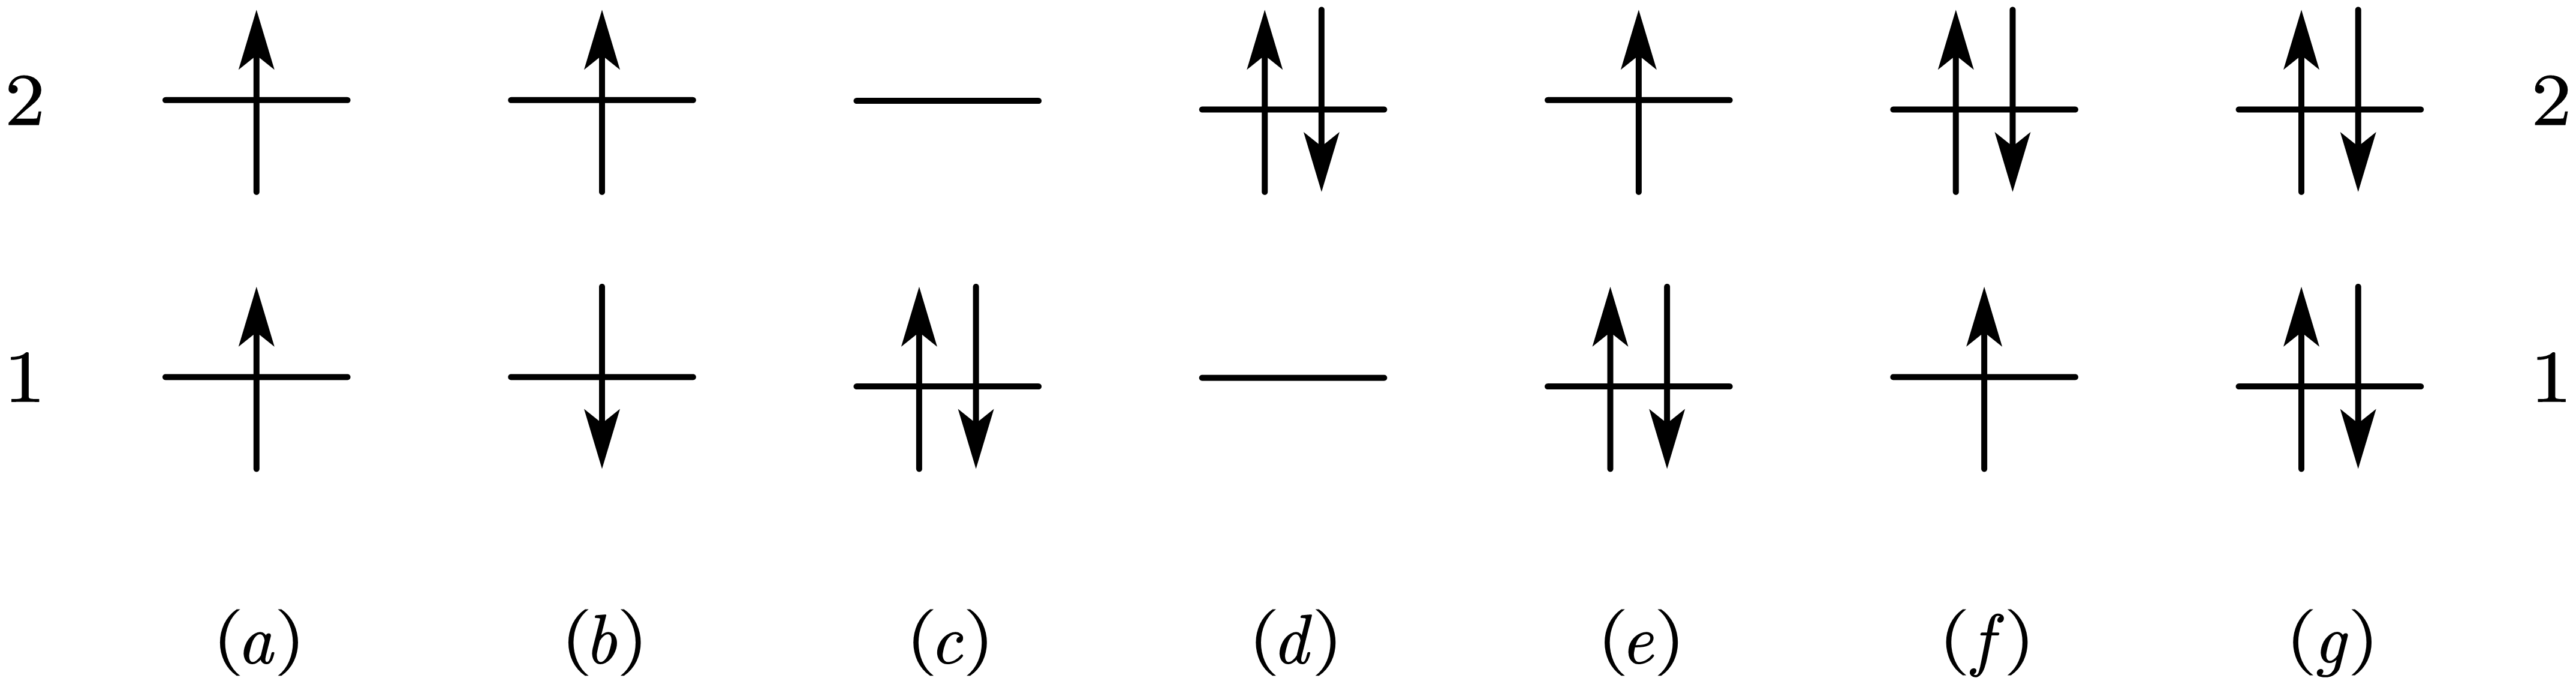
\includegraphics[scale=1.0]{89.png}
	\end{center}
	
	\begin{enumerate}
	
	\item[a.] $h_{11} + h_{22} +  J_{12} - K_{12}$.
	
	\item[b.] $h_{11} + h_{22} +  J_{12}$.
	
	\item[c.] $2h_{11} +  J_{11}$.
	
	\item[d.] $2h_{22} +  J_{22}$.
	
	\item[e.] $2h_{11} + h_{22} +  J_{11} + 2J_{12} - K_{12}$.
	
	\item[f.] $2h_{22} + h_{11} +  J_{22} + 2J_{12} - K_{12}$.
	
	\item[g.] $2h_{11} + 2h_{22} +  J_{11} +  J_{22} + 4J_{12} - 2K_{12}$.
	
	
	\end{enumerate}		
	
	\end{exercise}
	
	\begin{solution}
		2-23 so
	\end{solution}
	
	\section{Second Quantization}
	
	\subsection{Creation and Annihilation Operators and Their Anticommutation Relations}
	
	\begin{exercise}
	Show, using the properties of determinants, that
	\[
		( a^\dagger_1 a^\dagger_2 + a^\dagger_2 a^\dagger_1 ) | K \rangle = 0 
	\]
	for every $| K \rangle$ in set $\{ |\chi_1\chi_2\rangle , |\chi_1\chi_3\rangle , |\chi_1\chi_4\rangle , |\chi_2\chi_3\rangle , |\chi_2\chi_4\rangle , |\chi_3\chi_4\rangle \}$.
	\end{exercise}
	
	\begin{solution}
		2-24 so
	\end{solution}
	
	\begin{exercise}
	Show, using the properties of determinants, that
	\begin{align*}
		( a_1 a^\dagger_2 + a^\dagger_2 a_1 ) | K \rangle &= 0 , \\
		( a_1 a^\dagger_1 + a^\dagger_1 a_1 ) | K \rangle &= | K \rangle
	\end{align*}
	for every $| K \rangle$ in set $\{ |\chi_1\chi_2\rangle , |\chi_1\chi_3\rangle , |\chi_1\chi_4\rangle , |\chi_2\chi_3\rangle , |\chi_2\chi_4\rangle , |\chi_3\chi_4\rangle \}$.
	\end{exercise}
	
	\begin{solution}
		2-25 so
	\end{solution}
	
	\begin{exercise}
	Show using second quantization that $\langle \chi_i | \chi_j \rangle = \delta_{ij}$.
	\end{exercise}
	
	\begin{solution}
		2-26 so
	\end{solution}

	\begin{exercise}
	Given a state 
	\[
		| K \rangle = | \chi_1 \chi_2 \cdots \chi_N \rangle = a^\dagger_1 a^\dagger_2 \cdots a^\dagger_N | \rangle,
	\]
	show that $\langle K | a^\dagger_i a_j | K \rangle = 1$ if $i=j$ and $i \in \{ 1 , 2 , \cdots, N \}$, but is zero otherwise.
	\end{exercise}
	
	\begin{solution}
		2-27 so
	\end{solution}
	
	\begin{exercise}
	Let $|\Psi_0\rangle = | \chi_1 \cdots \chi_a \chi_b \cdots \chi_N \rangle$ be the Hartree-Fock ground state wave function. Show that
	\begin{enumerate}
	
	\item[a.] $a_r | \Psi_0 \rangle = 0 = \langle \Psi_0 | a^\dagger_r$.
	
	\item[b.] $a^\dagger_a | \Psi_0 \rangle = 0 = \langle \Psi_0 | a_a$.
	
	\item[c.] $| \Psi^r_a \rangle = a^\dagger_r a_a | \Psi_0 \rangle $.
	
	\item[d.] $\langle \Psi^r_a | = \langle \Psi_0 | a^\dagger_a a_r$.
	
	\item[e.] $| \Psi^{rs}_{ab} \rangle = a^\dagger_s a_b a^\dagger_r a_a | \Psi_0 \rangle = a^\dagger_r a^\dagger_s a_b  a_a | \Psi_0 \rangle $.
	
	\item[f.] $\langle \Psi^{rs}_{ab} | = \langle \Psi_0 | a^\dagger_a a_r a^\dagger_b a_s = \langle \Psi_0 | a^\dagger_a a^\dagger_b a_s a_r$.
	
	\end{enumerate}
	\end{exercise}
	
	\begin{solution}
		2-28 so
	\end{solution}
	
	\subsection{Second-Quantized Operators and Their Matrix Elements}
	
	\begin{exercise}
	Let $|\Psi_0 \rangle$ = $| \chi_1 \chi_2 \rangle$ = $a^\dagger_1 a^\dagger_2 | \rangle$ be the Hartree-Fock wave function for minimal basis $\ce{H2}$. Show using second quantization that
	\[
		\langle \Psi_0 | \mathscr{O}_1 | \Psi_0 \rangle = \sum_{ij} \langle i | h | j \rangle \langle \Psi_0 | a_2 a_1 a^\dagger_i a_j a^\dagger_1 a^\dagger_2 | \Psi_0 \rangle = \langle 1 | h | 1 \rangle + \langle 2 | h | 2 \rangle.
	\]
	\end{exercise}
	
	\begin{solution}
		2-29 so
	\end{solution}
	
	\begin{exercise}
	Show that
	\[
		\langle \Psi^r_a | \mathscr{O}_1 | \Psi_0 \rangle = \sum_{ij} \langle i | h | j \rangle \langle \Psi_0 | a^\dagger_a a_r a^\dagger_i a_j | \Psi_0 \rangle = \langle r | h | a \rangle
	\]
	by moving $a^\dagger_a$ and $a_r$ to the right.
	\end{exercise}
	
	\begin{solution}
		2-30 so
	\end{solution}
	
	\begin{exercise}
	Show that
	\[
		\langle \Psi^r_a | \mathscr{O}_2 | \Psi_0 \rangle = \sum_b^N \lr{rb}{ab}.
	\]
	{\it Hint}: first show that
	\begin{align*}
		\langle \Psi_0 | a^\dagger_a a_r a^\dagger_i a^\dagger_j a_l a_k | \Psi_0 \rangle &= \delta_{rj} \delta_{al} \langle \Psi_0 | a^\dagger_i a_k | \Psi_0 \rangle - \delta_{rj} \delta_{ak} \langle \Psi_0 | a^\dagger_i a_l | \Psi_0 \rangle \\
		&\hspace{2em} + \delta_{ri} \delta_{ak} \langle \Psi_0 | a^\dagger_j a_l | \Psi_0 \rangle - \delta_{ri} \delta_{al} \langle \Psi_0 | a^\dagger_j a_k | \Psi_0 \rangle
	\end{align*}
	then refer to Exercise 2.27.
	\end{exercise}
	
	\begin{solution}
		2-31 so
	\end{solution}
	
	\section{Spin-Adapted Configurations}
	
	\subsection{Spin Operators}
	
	\begin{exercise}
	a) Derive (2.247) from (2.245); b) Derive (2.248).
	\end{exercise}
	
	\begin{solution}
		2-32 so
	\end{solution}
	
	\begin{exercise}
	Find the $2 \times 2$ matrix representations of $s^2$, $s_z$, $s_+$, and $s_-$ in the basis $|\alpha\rangle$, $|\beta\rangle$. Verify the identities analogous to (2.248a,b) for these matrix representations.
	\end{exercise}
	
	\begin{solution}
		2-33 so
	\end{solution}
	
	\begin{exercise}
	Using the commutation relations (2.242), show that $[s^2, s_z]$ = 0.
	\end{exercise}
	
	\begin{solution}
		2-34 so
	\end{solution}
	
	\begin{exercise}
	Consider an operator $\mathscr{A}$ that commutes with the Hamiltonian. Suppose $|\Phi\rangle$ is an eigenfunction of $\mathscr{H}$ with eigenvalue $E$. Show that $\mathscr{A}|\Phi\rangle$ is also an eigenfunction of $\mathscr{H}$ with eigenvalue $E$. Thus if $|\Phi\rangle$ is (energetically) nondegenerate, then $\mathscr{A}|\Phi\rangle$ is at most a constant multiple of $|\Phi\rangle$ (i.e., $\mathscr{A}|\Phi\rangle = a|\Phi\rangle$) and hence $|\Phi\rangle$ is an eigenfunction of $\mathscr{A}$. In case of degeneracies, we can always construct appropriate linear combinations of the degenerate eigenfunctions of $\mathscr{H}$ that are also eigenfunctions of $\mathscr{A}$.
	\end{exercise}
	
	\begin{solution}
		2-35 so
	\end{solution}
	
	\begin{exercise}
	Given two nondegenerate eigenfunctions of a hermitian operator $\mathscr{A}$ that commutes with $\mathscr{H}$, i.e., $\mathscr{A} | \Psi_1 \rangle = a_1 | \Psi_1 \rangle$, $\mathscr{A} | \Psi_2 \rangle = a_2 | \Psi_2 \rangle$, $a_1 \neq a_2$, show that $\langle \Psi_1 | \mathscr{H} | \Psi_2 \rangle = 0$. Thus the matrix element of the Hamiltonian between, say, singlet and triplet spin-adapted configurations is zero.
	\end{exercise}
	
	\begin{solution}
		2-36 so
	\end{solution}
	
	\begin{exercise}
	Prove Eq.(2.254). {\it Hint:} Use expansion (2.115) for a Slater determinant and note that $\mathscr{S}_z$, since it is invariant to any permutation of the electron labels, commutes with $\mathscr{P}_n$.
	\end{exercise}
	
	\begin{solution}
		2-37 so
	\end{solution}
	
	\subsection{Restricted Determinants and Spin-Adapted Configurations}
	
	\begin{exercise}
	Prove Eq.(2.256. {\it Hint}: 1) $\mathscr{S}^2 = \mathscr{S}_- \mathscr{S}_+ + \mathscr{S}_z + \mathscr{S}^2_z$,  2) as a result of Eq.(2.254) it is sufficient to show $\mathscr{S}_+ | \psi_i \bar{\psi}_i \cdots \rangle$ = 0, 3) use expansion (2.115) for the determinant, and note the $\mathscr{S}_+$ commutes with the permutation operator, 4) $s_+ \psi_\alpha $ = 0, 5) finally, $s_+ \psi_\beta = \psi_\alpha $, but the determinant vanishes because it has two identical columns.
	\end{exercise}
	
	\begin{solution}
		2-38 so
	\end{solution}
	
	\begin{exercise}
	Using $\mathscr{S}^2 = \mathscr{S}_- \mathscr{S}_+ + \mathscr{S}_z + \mathscr{S}^2_z$, show that $|{}^1 \Psi^2_1 \rangle$ is a singlet while $|{}^3 \Psi^2_1 \rangle$, $| \Psi^{\bar 2}_1 \rangle$ and $| \Psi^2_{\bar{1}} \rangle$ are triplets.
	\end{exercise}
	
	\begin{solution}
		2-39 so
	\end{solution}
	
	\begin{exercise}
	Show that
	\begin{align*}
		\langle {}^1 \Psi^2_1 | \mathscr{H} | {}^1 \Psi^2_1 \rangle &= h_{11} + h_{22} + J_{12} + K_{12} , \\
		\langle {}^3 \Psi^2_1 | \mathscr{H} | {}^3 \Psi^2_1 \rangle &= h_{11} + h_{22} + J_{12} - K_{12} .
	\end{align*}
	Note that the energy of the triplet is lower than the energy of the singlet. Why is this to be expected from the space parts of the two wave functions?
	\end{exercise}
	
	\begin{solution}
		2-40 so
	\end{solution}
	
	\subsection{Unrestricted Determinants}
	
	\begin{exercise}
	Consider the determinant $| K \rangle = |\psi_1^\alpha \bar{\psi}^\beta_1 \rangle$ formed from {\it nonorthogonal} spatial orbitals, $\langle \psi^\alpha_1 | \psi^\beta_1 \rangle = S^{\alpha\beta}_{11}$. 
	\begin{enumerate}
	
	\item[a.] Show that $| K \rangle$ is an eigenfunction of $\mathscr{S}^2$ only if $\psi^\alpha_1 = \psi^\beta_1$.
	
	\item[b.] Show that $\langle K | \mathscr{S}^2 | K \rangle$ = 1 - $|S^{\alpha\beta}_{11}|^2$ in agreement with Eq.(2.271).	
	
	\end{enumerate}
	\end{exercise}
	
	\begin{solution}
		2-41 so
	\end{solution}
	


\end{document}